% THIS IS SIGPROC-SP.TEX - VERSION 3.1
% WORKS WITH V3.2SP OF ACM_PROC_ARTICLE-SP.CLS
% APRIL 2009
%
% It is an example file showing how to use the 'acm_proc_article-sp.cls' V3.2SP
% LaTeX2e document class file for Conference Proceedings submissions.
% ----------------------------------------------------------------------------------------------------------------
% This .tex file (and associated .cls V3.2SP) *DOES NOT* produce:
%       1) The Permission Statement
%       2) The Conference (location) Info information
%       3) The Copyright Line with ACM data
%       4) Page numbering
% ---------------------------------------------------------------------------------------------------------------
% It is an example which *does* use the .bib file (from which the .bbl file
% is produced).
% REMEMBER HOWEVER: After having produced the .bbl file,
% and prior to final submission,
% you need to 'insert'  your .bbl file into your source .tex file so as to provide
% ONE 'self-contained' source file.
%
% Questions regarding SIGS should be sent to
% Adrienne Griscti ---> griscti@acm.org
%
% Questions/suggestions regarding the guidelines, .tex and .cls files, etc. to
% Gerald Murray ---> murray@hq.acm.org
%
% For tracking purposes - this is V3.1SP - APRIL 2009

\documentclass{acm_proc_article-sp}

\usepackage{url} % for url citation
\usepackage{epstopdf}

\begin{document}

\title{Cloud Computing Data Capsule for Non-consumptive Text Analysis}

\numberofauthors{8}
\author{
\alignauthor
Jiaan Zeng \\
       \affaddr{School of Informatics and Computing Indiana University}\\
       \email{jiaazeng@indiana.edu}
\alignauthor
Guangchen Ruan \\
       \affaddr{School of Informatics and Computing Indiana University}\\
       \email{gruan@indiana.edu}
\alignauthor 
Alexander Crowell \\
       \affaddr{Department of Computer Science and Engineering University of Michigan}\\
       \email{crowella@umich.edu}
\and  % use '\and' if you need 'another row' of author names
\alignauthor 
Atul Prakash \\
       \affaddr{Department of Computer Science and Engineering University of Michigan}\\
       \email{aprakash@umich.edu}
% 5th. author
\alignauthor Beth Plale \\
       \affaddr{School of Informatics and Computing Indiana University}\\
       \email{plale@indiana.edu}
}

\maketitle
\begin{abstract}
As digital archives grow in size, the interest by humanities and informatics
researchers alike increases in computational investigation of a corpus.  The
cloud computing model of ``data as a service'' which co-locating computation with
a data collection of value, allows for scales of computational analysis that
far exceeds what a desktop machine can provide. However, when data collections
are protected, such as digitized books are through copyright, there are
additional challenges to provisioning an analytical framework. We investigate
issues in text analysis on a protected corpus in a cloud environment that
prevents reconstruction of part or whole of the corpus.  The proposed framework
makes use of a novel notion of "data capsule" to enforce non-consumptive
research policy using virtual machines.
\end{abstract}


% A category with the (minimum) three required fields
\category{H.3.4}{Systems and Software}{Distributed Systems}[Cloud Computing, Data Capsules]
%A category including the fourth, optional field follows...
\category{K.6.m}{Miscellaneous}{Security}[Non-consumptive Research]

\terms{Architecture, Design, Implementation}

\keywords{Cloud computing, Large-scale Text Mining, Non-consumptive Research, Data Capsules} % NOT required for Proceedings

\section{Introduction}
As increasing amounts of digitized text become available from sources such as university libraries, researchers encounter access to more material than they could ever hope to read in life time, creating opportunities for new forms of research. For example, research has checked literary critic Ian Watts' claims against 3,600 novels written between the 18th and 19th centuries \cite{Example}. While this tedious task could be carried out by hand, digitized texts coupled with text mining tools, enables new discoveries.  One can apply topic modeling such as Latent Dirichlet allocation (LDA)~\cite{LDA}) at the book level to narrow from millions of texts to a few thousand, then page level LDA to zero down to relevant pages, effectively expanding the reach of research investigation of the informatics or digital humanities researcher.

Texts digitized from research libraries have restrictions on their use; most obviously copyright for content that is post about 1923.  While most in the legal community would agree that text mining qualifies as fair use, the text mining cannot as a byproduct leak entire books to web pages.  This kind of limited analytical use on the data we call \textit{non-consumptive research}.  Non-consumptive research we define as \textit{No action or set of actions on the part of users, either
acting alone or in cooperation with other users over the duration of one or multiple sessions can result in sufficient information gathered from a collection of copyrighted works to reassemble pages from the collection.}

In this paper we propose a novel solution to non-consumptive research that uses a data capsule approach~\cite{Borders:2009:PCD:1855768.1855791} preventing misuse.  The work is being carried out in the context of the HathiTrust Research Center~\cite{HTRC}, a set of software and services that currently provide text analysis capability over public domain books.  HTRC is in the process of securing access to 12 million volumes of text data and images from research libraries across the country.

Text analytics over a large corpus of sensitive data poses challenges for several reasons. First, text mining tools vary in their computational demand. Analysis could take the form of simple access to a database of features; could involve a linear traversal through digitized text; or could be a computationally intensive natural language processing task like LDA.    Second, while high performance computing (HPC) gives a user resources dynamically based on workload, HPC systems remain largely batch oriented which is out of phase with digital humanities researcher requiring high levels of interaction with texts. The cloud computing data-as-service model avoids the problem of limited interactivity. Third, and the biggest challenge of the three, is that digitized texts can have restrictions on their access.  Allowing interactive access on texts user algorithms run directly on copyrighted texts opens a vulnerable channel that non-consumptive constraint may be violated.

We propose a non-consumptive cloud framework for data analytics on sensitive corpora.   Using a remote virtual machine (VM) model, researchers can build a VM configured with software and tooling based on their need. Once an analysis is finished, the VM is wiped out and resources released for other users to share. VMs offer no inherent protection, however.  Our approach extends the virtual machine by turning it into a \textit{data capsule}\cite{Borders:2009:PCD:1855768.1855791} that prevents leakage of copyrighted content in the event that the VM is compromised or data analysis routines malicious.  The HTRC Data Capsule provides the virtual machine with two modes: a maintenance mode during which a user can access the network and install software freely, but cannot access copyrighted data; and secure mode where copyrighted texts become accessible to user while the network access and file system access is highly constrained. In the latter mode, users are allowed only  access to a predefined set of network addresses and write to a specific volume which is only visible in secure mode. Every other changes user made to the system in secure mode, except for the ones made to special volume, is lost when mode is switched from secure to maintenance. This is to guard against the situation that copyrighted texts is saved in VM in secure mode and copied out through network in maintenance.

This paper introduces the architecture and design of the HTRC Data Capsule.  The research question driving HTRC Data Capsule imposes five major requirements as follows:

\begin{itemize}
\item Non-consumptive research: that is, provides safe handling of large volumes of data, and
can ensure that the read restrictions of the definition hold
\item Openness: users are not limited to using a known set of algorithms, and instead are
expected to experiment with their own algorithms
\item Efficiency: It is not possible to analyze algorithms for conformance prior to
execution
\item Low cost and scale:  Run at large-scale and low cost to users
\item  Long term and broad value:  framework is designed for adoption for other
purposes
\end{itemize}

%Jiaan,  these above are the requirements from the proposal.  These replace the requirements that were in Sec 3, which were much more implementation focused and not appropriate for a research paper.

This paper is organized as follows: Section \ref{title:related} summaries related work and \ref{title:overview} presents an overview of HTRC and data capsule, and identifies the design requirements for our system. Section \ref{title:design} describes details of our system design and implementation. Section \ref{title:future} outlines future work and section \ref{title:conclusion} concludes.

\section{Related Work} \label{title:related}

Research that leverages the power of cloud computing for text analysis has been done. Teregowda et al. employ cloud computing as underlying infrastructure for CiteSeerX, which is a public search engine and digital library for scientific and academic papers \cite{Teregowda:cloud}. Rosenthal et al. propose LOCKSS for digital preservation; LOCKSS uses a cloud model in their digital preservation system~\cite{Rosenthal:preservation}. Our system differs from those systems because of the protection requirements of non-consumptive research in the cloud platform.

There are numerous cloud platforms that support IaaS, either commercially or in open source. Amazon EC2 \cite{EC2} is probably the most well-known IaaS platform, but there is Eucalyptus \cite{Nurmi:2009:EOC:1577849.1577895}, and OpenStack \cite{OpenStack}. Researchers investigated different cloud platforms \cite{Sempolinski:cloud,vonLaszewski:2012:CMC:2353730.2353779}. We do not build our system on existing open source cloud platforms for two reasons: first, existing cloud platforms introduce numerous complexities for the data capsule which has to enforce the non-consumptive research policy in the VM. The complexities stem from avoiding imposing unnecessary burdens on the digital humanities researcher. For example, the researcher should not need to configure a software defined network to run her text mining algorithms. Second, existing cloud platforms are designed for general purpose and expose many vulnerable channels. For example, allowing user to configure network would pose significant threats to our systems. Therefore, instead of using existing cloud platform, we build a cloud framework around data capsule, which satisfies digital humanities researchers\rq need and non-consumptive research requirement. Our research also illuminates the path that data capsule could potentially be applied to more general cloud platforms.

Data capsules \cite{Borders:2009:PCD:1855768.1855791} is a mechanism for
containing sensitive data within a virtualized environment with the goal of
minimizing the available channels to leak that data.  Although data capsules
provide no guarantees on the integrity of the stored data -- which could be
modified or deleted by an attacker -- this poses little issue when data 
capsules is applied to non-consumptive research, where the copyrighted source
data can simply be made read-only.  Additionally, the data capsules design
is well-suited to non-consumptive research, in that it is able to maintain
strong security guarantees on the sensitive data while being highly permissive
to users, who may need to install custom software or perform other actions that
would require the granting of many privileges in a normal environment.  The
application of data capsules we present in this paper currently does not
provide the same level of protection against covert channels that is provided
in the original data capsules system, but improvements in the implementation
are being made that will eventually provide greater protection than that given
in the original work.

\section{Overview} \label{title:overview}
This section presents background of the HathiTrust Research Center software and services, data capsule and identifies threat model as well as design requirements for our system.

\subsection{HathiTrust Research Center Background} \label{subtitle:background}
The HathiTrust Research Center is a set of software and services to carry out computational analysis using digitized books from the HathiTrust Digital Library for research and educational use.
Figure \ref{fig:htrc} is a cartoon diagram of the system.  A researcher accesses the system through one or more front ends (shown on right).  The system in its simplest form satisfies a user need by constructing for the user a \textit{Workset} representing selected text mining tools, selected subsets of data from either the HathiTrust digital repository, or from feature sets that have been extracted in advance, and data from other sources.   This Workset bundle is executed on a large-scale compute resource.   As is shown by the arrow pointing to both compute resource and front end (complexity hiding interface), text analysis is a highly interactive process, thus challenging the use of HPC resources shown, even if, like Big Red 2 at Indiana University, they are architected to handle data-intensive computations.  The HTRC system is modularly architected using a web services paradigm (i.e., REST interfaces).  It utilizes a Solr index, Cassandra noSQL store, both of which are sharded across half-dozen machines for higher replicability and availability.  Analytical tools include the SEASR suite of text mining tools, with ongoing extension of support to R and i-Python.

The HTRC architecture uses OAuth2 authentication and has an auditing service.   While this architecture is adequate for analysis algorithms that have been vetted by HTRC, it cannot support analysis algorithms that originate with an external researcher.  This latter issue is the purview of the HTRC Data Capsule.


\begin{figure}[tbh]
  \centering
  \includegraphics[scale=0.3]{figures/htrc}
  \caption{Functional diagram of HathiTrust Research Center software and services}
  \label{fig:htrc}
\end{figure}

\subsection{Data Capsules}

Data capsules is a system developed by Borders et al.
\cite{Borders:2009:PCD:1855768.1855791} that allows privileged access to
sensitive data while also restricting the channels through which that data can
be released.  Capsules uses virtual machine snapshotting and simple
policy-based restriction mechanisms to allow a user to enter a ``secure'' mode,
where network and other data channels are restricted in exchange for access to
the data being protected.  After using the protected data, when the user
returns to normal use of the system, which we call ``maintenance'' mode, all
changes to the system except those made to the designated secure data are
forgotten, and the system returns to the state it was in before the switch to
secure mode, thereby regaining full Internet access and the ability to make
persistent changes to the virtual machine, such as installing software.  In
this way, network and storage channels cannot be used to leak the sensitive
data.  This usage model is readily applicable to non-consumptive research, in
that a researcher can administer their system (e.g. install any required
software tools) and then switch to ``secure'' mode to perform their analysis.  

Because data capsules was originally developed with use on a personal
machine in mind, it had to be adapted and extended to work within the HTRC
cloud environment. In HTRC, sensitive data is copyrighted text that is exposed
through a Restful web service API instead of within a machine. Data capsules
manages the network channel between virtual machines and the web services
serving data to them. In consideration of potential future HTRC services,
data capsules has a flexible network control mechanism that allows network
policies for different modes to be written by administrators. 

Additionally, in order to provide a cloud environment across multiple machines
and to a large number of researchers, there is a need for another layer on top
of data capsules that coordinates different machines. We therefore
implemented a web service layer that is responsible for management of virtual
machines (e.g., resource allocation, request scheduling, status maintenance)
above the data capsules layer.  Section \ref{title:design} gives details of
the design and implementation of data capsules and the web service layer in
the context of HTRC.

\subsection{Threat Model}

Under our usage model, users access the copyrighted data through remotely
accessed virtual machines that read the data from a network-accessed data
service.  The virtual machine presented by the user is not a part of the trusted
computing base (TCB).  We assume the possibility of malware being installed as
well as other remotely initiated attacks on the VM.  These attacks could
potentially compromise the entire operating system and install a rootkit that
are undetectable to the end user.  The end users themselves are considered to
act in good faith, but this does not preclude the possibility of them
unwittingly allowing the system to be compromised.  We believe this is a
reasonable assumption since users are required to sign a legal agreement before
using our system.  Beyond the virtual machine itself, the virtual machine
manager (VMM) and the host it runs on are both trusted, and fall within the TCB.
This includes system services that enforce network and data access policies for
the virtual machines.  Finally, the HTRC Data service itself is also a part of
the TCB.

Users have VNC access to their virtual machines so that they have a graphical
interface to the machine.  However, this access does admittedly provide a
channel for potential data leak.  For now, we apply our assumption that the end
user acts in good faith, and also assume that they are the only one accessing
the virtual machine.  For future work, we can use analysis of the channel as a
means to automatically detect potential abuses of it for data leak purposes.
Additionally, a channel is provided to the user for releasing results when their
research is complete.  Although we currently intend to allow released results to
be downloaded via a link sent to the end user's email inbox, we note that the
released data could also be subjected to manual or automated review to detect
potential abuses.  We also leave this for future work.

Another potential threat is that of covert channels between virtual machines
that run on the same host machine.  For instance, a virtual machine running in
secure mode could possibly make use of such covert channels to leak data to a
coresident virtual machine running in maintenance mode, which can in turn leak
the data anywhere it pleases.  We acknowledge that this could pose a serious
threat, but leave addressing it for future work.

\section{Design and Implementation} \label{title:design}

 The high level architecture of the HTRC Data Capsule, see Figure \ref{fig:architecture}, consists of three layers shown bottom to top: a physical layer, a web service layer and web front-end layer. The physical layer consists of physical machines and hypervisor software that run the virtual machines of the data capsule. It also includes the data capsule implementation which is scripts that wrap hypervisor commands to perform multiple tasks. Database, image store and volume store also sit in this layer. The database is used by the web service layer to maintain persistent states for virtual machines and different operations.

Virtual machine images as well as secure volumes locate on NFS, a distributed file system. The web service layer is the central controller of the system. It is responsible for resource allocation, request scheduling, state maintenance, and failover on physical layer. It also has an audit component to log user activities. Finally we expose the system through the web font end layer. It consists of a web UI where user interacts with our system and a user authentication server which validates user identification. To validate user identity, we use OAuth 2.0 \cite{OAuth2} for user authentication.

\begin{figure}[ht]
  \centering
  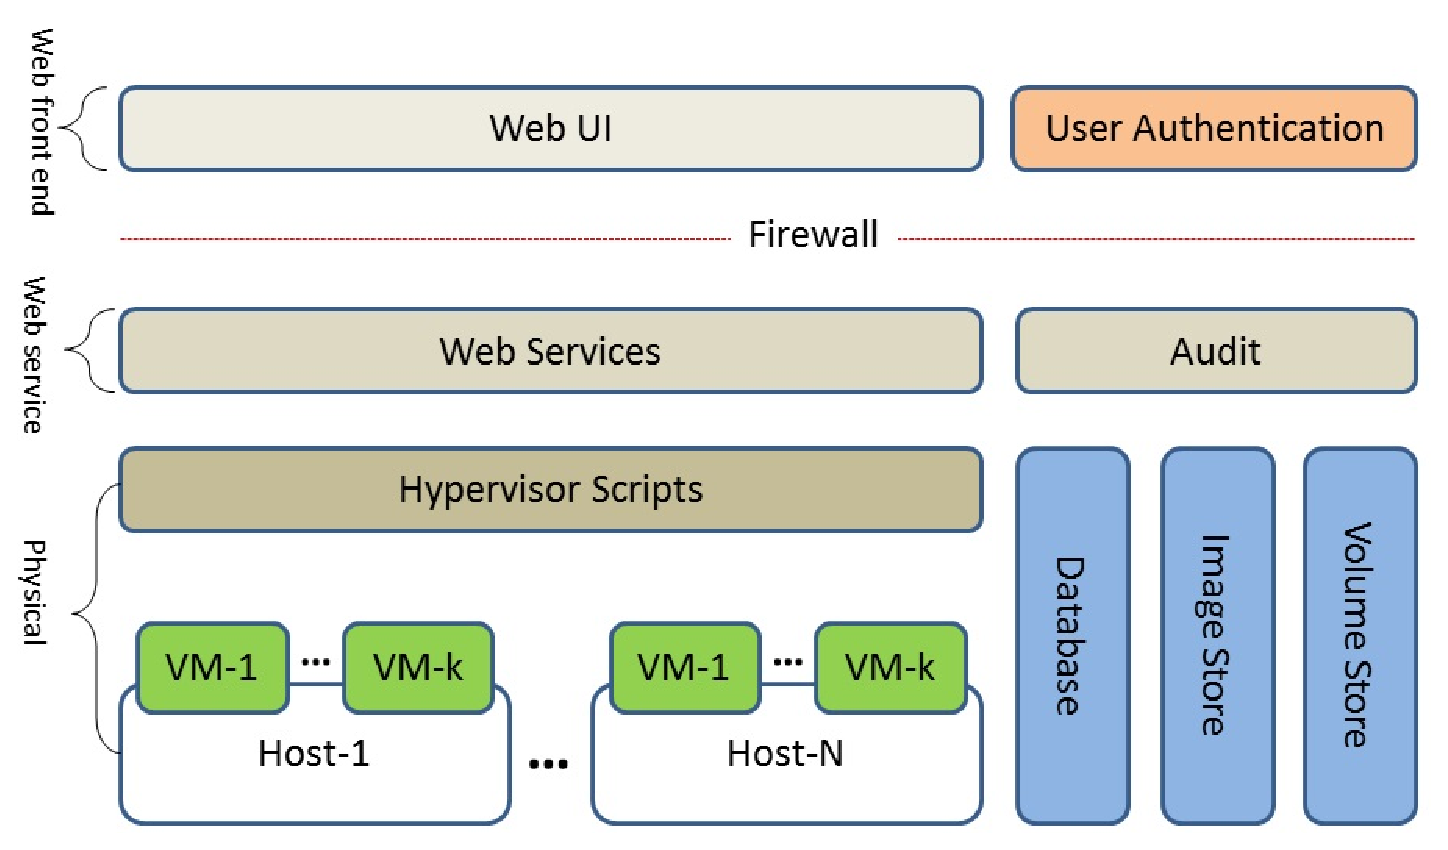
\includegraphics[scale=0.33]{figures/layers}
  \caption{HTRC Data Capsule architecture}
  \label{fig:architecture}
\end{figure}


\subsection{Workflows}

There are three major control flows within the HTRC Data Capsule system:   virtual machine creation, authentication, and VM access.  Each are described in turn.

\subsubsection{Virtual machine operations} \label{subsubtitle:control}
Figure \ref{fig:control} describes the control flow in our system. First user logs into web UI, which delegates the authentication to OAuth 2 server which validates user login credentials. Details of user authentication is presented in section \ref{subsubtitle:auth}. Upon validation success, user can manipulate the VM through the web UI. We use VM creation request as an example here. The UI forwards the request along with an authentication token to web service. When web service receives the request, it validates the token against OAuth 2 server again. The reason for double validation is web UI might be compromised and web service needs to validate requests coming from web UI. If validation successes, web service will prepare to invoke corresponding hypervisor script. It makes scheduling decision on which host to launch VM, allocates ports for VM, retrieves image information from database, and etc. Once the preparation is done, it will call hypervisor script remotely to launch a VM on a particular host, monitor the response and update VM state in database. Meanwhile web service will return user the information required to log into VM, e.g., VNC port. Other VM operations (shutdown, delete, launch, switch mode from one another) follow the same path described above.

\begin{figure}[ht]
  \centering
  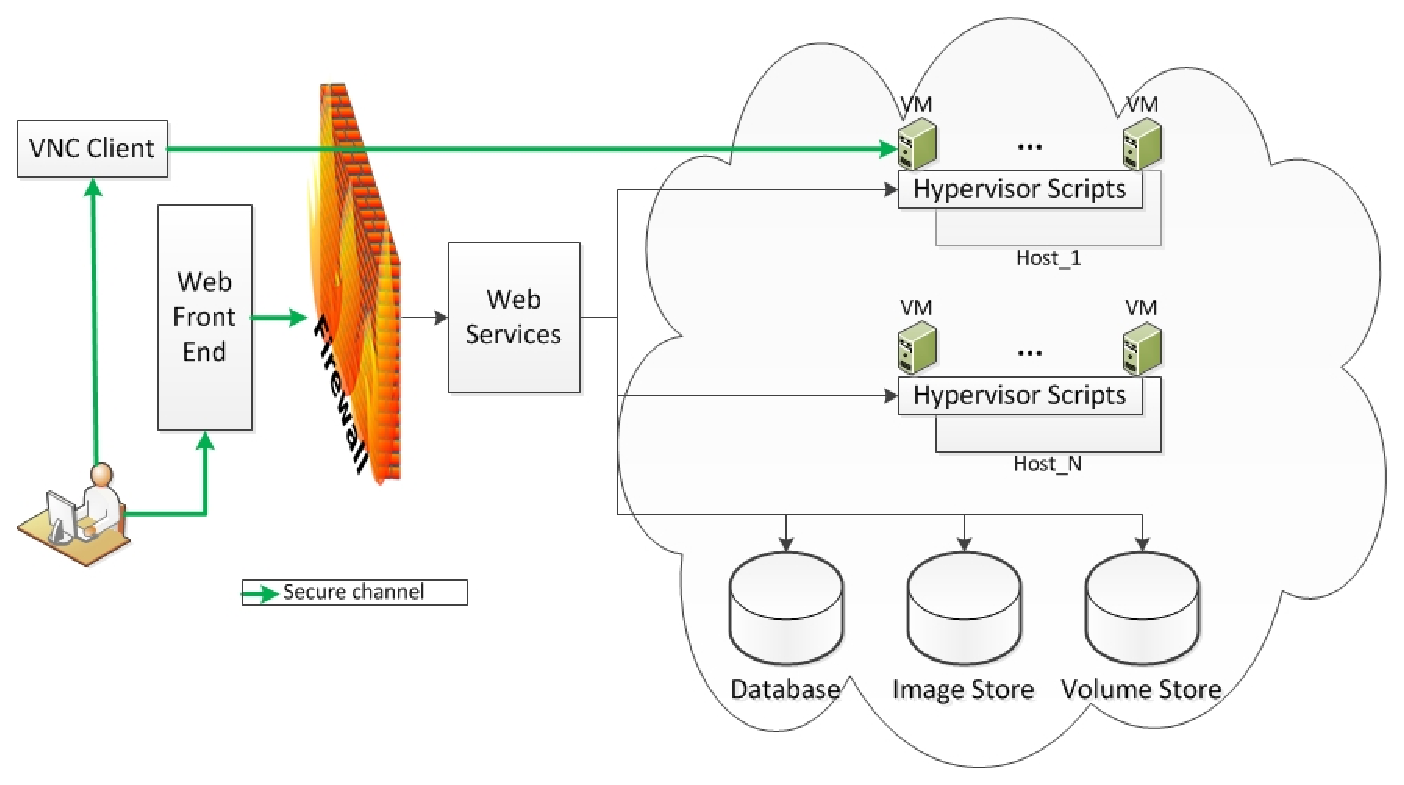
\includegraphics[scale=0.35]{figures/workflow-control}
  \caption{System control flow.}
  \label{fig:control}
\end{figure}

\subsubsection{Authentication} \label{subsubtitle:auth}
We use OAuth 2.0 as our authentication protocol \cite{OAuth2}. A dedicated server with OAuth 2.0 implementation is setup to authenticate user. Following steps summarize the authentication procedure as presented in Figure \ref{fig:auth}.
\begin{enumerate}
  \item User requests login to the web UI;
  \item Web UI redirects user to the authentication server which requires user login credentials;
  \item Authentication server sends a token back to web UI to indicate validation successes;
  \item After receiving the token, web UI can forward user requests to web service along with the token;
  \item Web service layer would make sure that the request is valid for the given user through validating token against authentication server. Web service layer would also use the token to retrieve the user's identity from authentication server.
\end{enumerate}

\begin{figure}[ht]
  \centering
  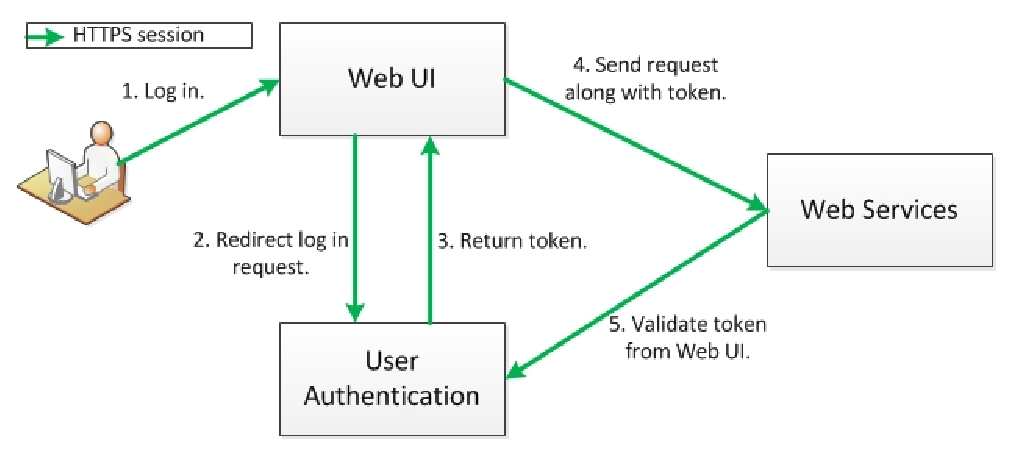
\includegraphics[scale=0.5]{figures/workflow-authentication}
  \caption{Authentication flow.}
  \label{fig:auth}
\end{figure}

\subsubsection{Virtual machine access}

Section \ref{subsubtitle:control} presents an overview of different VM operations. This section focuses on the mechanism we provide to user to access VM. There are two possibilities that copyrighted data may leak from our system during user access. One of them is through network. For one VM, we intend to block arbitrary network access when a user accesses copyrighted data, while keeping network open for the user to download and configure software environment when she does not access copyrighted data. The data capsule provides two VM mode, i.e. maintenance mode and secure mode, to support different network control for the same VM. In maintenance mode, user can access network without any constrains, although the HTRC data service is blocked by firewall policy. In secure mode, user can only access HTRC data service. Any other network accesses are denied. Figure \ref{fig:vmaccess} gives an example. First user creates and starts a VM through the web UI as described in section \ref{subsubtitle:control}. After the VM is up and running, the user can log in to it through any VNC client with proper information provided from web UI, e.g., host name and port number. Note that VNC session is the only channel that user can access VM in secure mode. We block SSH traffic, which is a typical way to access VM in most cloud platforms e.g., Amazon EC2, OpenStack, because it allows user to copy data out by scp command. By default, user logs into VM in maintenance mode. User can install software from internet, upload programs from her desktop, and etc. If user wants to access HTRC Data service, she needs to switch VM mode from maintenance to secure through web UI. In practice, VNC screen will be frozen for a short time (usually 2 to 5 seconds) during the mode switch. In secure mode, user does not have network access except for HTRC Data service.

The other possibility of copyrighted data leakage is to copy data from secure mode to maintenance mode in local disk and leak through network in maintenance mode. In secure mode, copyrighted data may be copied from HTRC Data service in local disk. When VM is switched to maintenance mode, the copyrighted data in local disk is visible in maintenance mode and can be copied out through network. To prevent such leakage, data capsule checkpoints VM image before it goes to secure mode. That is to take a snapshot of the VM by using qemu command. When VM switches from secure mode to maintenance mode, data capsule restores the checkpoint, i.e, the snapshot image, through qemu command. Therefore, all the data written to VM local disk in secure mode will be wiped out when VM switches from secure mode to maintenance mode. Meanwhile, to allow user to persist her data in secure mode, data capsule provides a secure volume, which is only visible in secure mode and shown as an external drive to the VM, to let user write data to. The secure volume stores data persistently and will be detached from VM when VM is in maintenance mode.

A typical workflow for a user to access the VM is depicted in figure \ref{fig:vmaccess}. First, the user creates and starts the VM through web UI. Second, user logs in to VM in maintenance mode through VNC client (step 1). Third, user configures software setting through internet (step 2). Forth, user switches VM mode from maintenance to secure, accesses HTRC Data service and writes data to secure volume (step 3, 4).

Final result release??

\begin{figure}[ht]
  \centering
  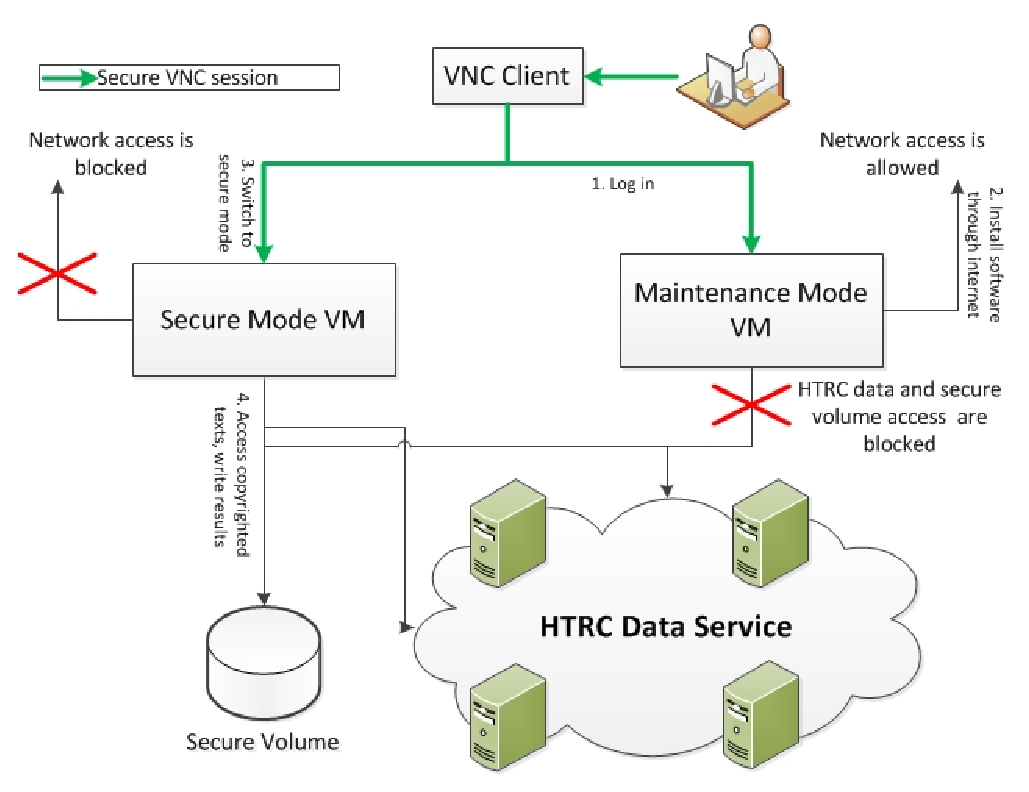
\includegraphics[scale=0.45]{figures/workflow-HTRCData}
  \caption{Virtual machine access flow.}
  \label{fig:vmaccess}
\end{figure}


\subsubsection{Final results review}

%Jiaan,  this section needs to tie back around and wrap in the requirements laid out in section 1.  The implementation requirements in Sec 3 are now gone.  In addressing the broader goals in Sec 1,  how well does the work so far address these requirements?  What's been done and what hasn't been addressed (for instance: we haven't tried for generality yet.)  This is still a 'towards' paper so can and should be honest about where we are and where open work still exists

Under construction.

First, the web front end and web service use OAuth 2.0 to authenticate user which denies unauthorized users. Second, web service coordinates a number of machines equipped with data capsule to provide a cloud environment and log all user activities. Through the log files, we are able to tell who did what. Third, the data capsule blocks network channels when VM is in secure mode so that no copy out can take place. Forth, researcher can manage and manipulate her virtual machines through a simple web UI which is more user friendly than a command line tool. Besides, researcher can log in to virtual machine through VNC which provisions GUI desktop instead of terminal. In addition, researcher is allowed to configure the hardware setting when creating the VM from web UI and software setting in VM in maintenance mode to meet her needs. These effects help lower the usage burdens for digital humanities researchers. Last but not least, the web service can setup a Hadoop cluster for researcher to run MapReduce jobs although more efforts are needed to configure data capsule properly in a MapReduce context. We leave it as future work.

\subsection{Implementation Details}

\subsubsection{Physical layer implementation}

The backend that manages virtual machines is implemented as a set of Linux
shell scripts that manage the \texttt{qemu} VMM in order to implement the
functionality of data capsules.  These scripts are remotely run by the web
service via a secure shell (SSH) connection.  \texttt{qemu} provides live
snapshotting functionality that serves an important role in realizing our
data capsules implementation.  When a user transitions to secure mode, a
snapshot is taken of the entire virtual machine state via the backend scripts,
and any further use of the system is recorded in memory and does not persist
upon shutdown or any other operation.  Upon return to maintenance mode, the
snapshot taken earlier is restored, and all system progress that followed it is
forgotten.

Virtual machines are isolated from the rest of the host's networking through the
use of a tap interface.  Their connection is then bridged to host networking.
Network policies for both modes are implemented using iptables rules.  These
rules can be written in custom policy files that can be specified on mode
switch, allowing for any arbitrary policy desired by the administrator.  In
addition to the policy rules, some basic rules are always enforced, for example
preventing communication between virtual machines residing on the same host.

\subsubsection{Web service layer implementation}
The web service is implemented as an asynchronous Restful service in Jersey framework []. Since operations in hypervisor layer usually take some time to finish, we decouple the response and actual execution to provide good responsiveness. For instance, when a start VM request arrives, web service returns \emph{start-pending} as VM state immediately rather than waits until VM startup finishes and returns \emph{start} state. The web service also takes into account failover on hypervisor layer. It automatically retries connection failure and timeouts long running ssh session. The web service is implemented in a multi-threaded way so that multiple operations on different VM can happen simultaneously.


\section{Future Work} \label{title:future}
We are in the process of implementing final results review mechanism. Once that part is in place, we expect to release our system to humanities researchers for use and get feedbacks from them. There are numerous next steps we can take. First, we intend to build MapReduce cluster automatically with data capsule in place to expand the utilization of data capsule. Second, we are interested in providing researchers with extractive features that comply with non-consumptive research policy. Potential qualified features include word frequency, term document matrix, etc. Third, we will investigate the approach of adding random noises to final result so that user is unable to reconstruct original texts while the accuracy of final results is bounded. For example, after adding noises, the lower bound of accuracy is 90\% which may be sufficient enough to researchers.

\section{Conclusion} \label{title:conclusion}

This paper proposes a cloud framework which complies with non-consumptive research policy to facilitate digital humanities research. The framework is built on top of data capsule and data capsule is extending to adapt to a cloud environment.  We present design details of the framework along with implementation details. Most parts of the system are implemented. We are in the process of implementing the final result review mechanism and plan to release our system to digital humanities researchers in the next couple of months.


%ACKNOWLEDGMENTS are optional
\section{Acknowledgments}
This research funded through a grant from the Alfred P. Sloan Foundation, grant \# xxxxxx
%ask Nicole to give you the grant number; I'm not finding it.   This needs to be the number the Sloan foundation knows, not IU's internal grant #

%
% The following two commands are all you need in the
% initial runs of your .tex file to
% produce the bibliography for the citations in your paper.
\bibliographystyle{abbrv}
\bibliography{sigproc}  % sigproc.bib is the name of the Bibliography in this case
% You must have a proper ".bib" file
%  and remember to run:
% latex bibtex latex latex
% to resolve all references
%
% ACM needs 'a single self-contained file'!
%
%APPENDICES are optional
%\balancecolumns

% That's all folks!
\end{document}
